\section{Evaluation}\label{sec:evaluation}
\begin{frame}[t]{NoC Configuration Tool}
	\begin{center}
		\includegraphics[width=0.75\linewidth]{images/evaluation/shocgentool.png}
	\end{center}
	\begin{itemize}
		\item<only@1> Graphical configuration tool to generate and compute scenarios at \textit{design time}
		
		\item<only@2> Implements SBR and RBR algorithms to populate routing entries
		
		\item<only@3> Performs routing entries, \textbf{\textit{FIZ/PIZ}} routing paths, and latency evaluations
		
		\item<only@4> Outputs the generated configuration to a SystemC simulation platform
	\end{itemize}
\end{frame}

%%%%%%%%%%%%%%%%%%%%%%%%%%%%%%%%%%%%%%%%%%
%%% EVALUATION CRITERIA %%%%%%%%%%%%%%%%%%
%%%%%%%%%%%%%%%%%%%%%%%%%%%%%%%%%%%%%%%%%%
\subsection{Evaluation Criteria}
\begin{frame}[t]{Evaluation Criteria}
	\begin{center}
		\resizebox{1.0\linewidth}{!}
		{
			\begin{tabular}{c|c|c|c|c}
				\toprule[2pt]
				Scenario & NoC Dimension (Columns $X$ Rows) & SBR Seeds & Segmentation Modes & Configurations per Scenario\\
				\midrule[1.5pt]
				NASA NAS & 13x13         & 169       & \emph{SBR} / \emph{SBR-SZA} &338 \\
				\hline
				Synth 1  & 6x4           & 24        & \emph{SBR} / \emph{SBR-SZA} &48  \\
				\hline
				Synth 2  & 10x6          & 60        & \emph{SBR} / \emph{SBR-SZA} &120 \\
				\midrule[1.5pt]
				\multicolumn{4}{r|}{Total:}                                        &506 \\
				\bottomrule[2pt]
			\end{tabular}
		}
	\end{center}
	
	\begin{itemize}
		\setlength{\itemsep}{1em}
		\item<only@1> Three scenarios evaluated: 2 synthetic and 1 based on a real application communication dependency trace
		
		\item<only@1> Evaluation consists of four preliminary steps
		\begin{itemize}[i]
			\setlength{\itemsep}{0.5em}
			\item<only@1> Seed for segment computation
			
			\item<only@1> SBR computation
			
			\item<only@1> RBR computation
			
			\item<only@1> Evaluation of obtained configuration
		\end{itemize}
		
		\setlength{\itemsep}{1em}
		\item<only@2> Three evaluations were performed:
		\begin{itemize}[i]
			\setlength{\itemsep}{0.5em}
			\item<only@2> Routing table scalability
			
			\item<only@2> \textbf{\textit{FIZ/PIZ}} occurrences
			
			\item<only@2> Latency estimation
		\end{itemize}
	\end{itemize}
\end{frame}

%%%%%%%%%%%%%%%%%%%%%%%%%%%%%%%%%%%%%%%%%%
%%% PRELIMINARY RESULTS %%%%%%%%%%%%%%%%%%
%%%%%%%%%%%%%%%%%%%%%%%%%%%%%%%%%%%%%%%%%%
\subsection{Preliminary Results}
\begin{frame}{Routing Table Scalability - Average Routing Tables Size}
	\begin{center}
		\begin{figure}
			\begin{subfigure}{0.49\linewidth}
				\includegraphics[width=1.0\linewidth]{charts/synth1/synth1-routing-tables-bits-bezier.eps}
			\end{subfigure}
			\begin{subfigure}{0.49\linewidth}
				\includegraphics[width=1.0\linewidth]{charts/synth2/synth2-routing-tables-bits-bezier.eps}
			\end{subfigure}
			\begin{subfigure}{0.49\linewidth}
				\includegraphics[width=1.0\linewidth]{charts/nasa/nasa-routing-tables-bits-bezier.eps}
			\end{subfigure}
		\end{figure}
	\end{center}
\end{frame}

\begin{frame}{Routing Table Scalability - Optimal Configuration Heatmap}
	\begin{center}
		\begin{figure}
			\begin{subfigure}{0.45\linewidth}
				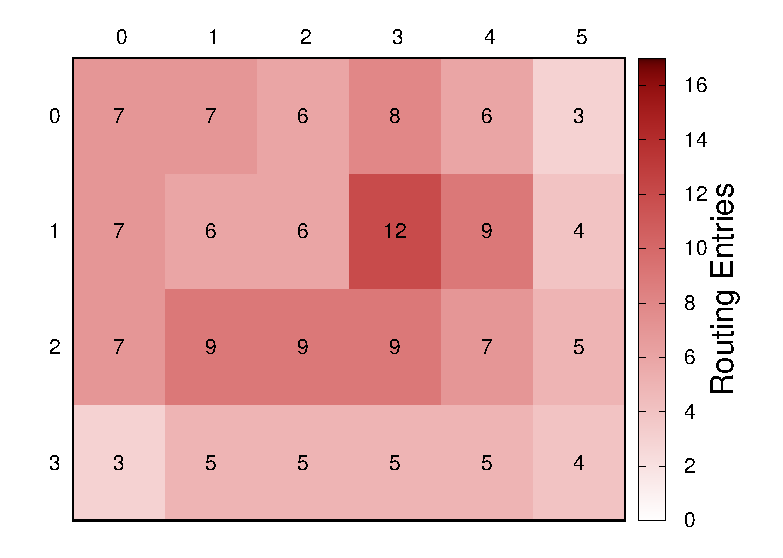
\includegraphics[width=1.0\linewidth]{charts/synth1/synth1-routing-tables-heatmap-sla-off-optimal.eps}
			\end{subfigure}
			\begin{subfigure}{0.45\linewidth}
				\includegraphics[width=1.0\linewidth]{charts/synth2/synth2-routing-tables-heatmap-sla-off-optimal.eps}
			\end{subfigure}
			\begin{subfigure}{0.45\linewidth}
				\includegraphics[width=1.0\linewidth]{charts/nasa/nasa-routing-tables-heatmap-sla-off-optimal.eps}
			\end{subfigure}
		\end{figure}
	\end{center}
\end{frame}

\begin{frame}{FIZ Occurrences}
	\begin{center}
		\begin{figure}
			\begin{subfigure}{0.49\linewidth}
				\includegraphics[width=1.0\linewidth]{charts/synth1/synth1-piz-routes-bezier.eps}
			\end{subfigure}
			\begin{subfigure}{0.49\linewidth}
				\includegraphics[width=1.0\linewidth]{charts/synth2/synth2-piz-routes-bezier.eps}
			\end{subfigure}
			\begin{subfigure}{0.49\linewidth}
				\includegraphics[width=1.0\linewidth]{charts/nasa/nasa-piz-routes-bezier.eps}
			\end{subfigure}
		\end{figure}
	\end{center}
\end{frame}

\begin{frame}{Latency Variation}
	\begin{center}
		\begin{figure}
			\begin{subfigure}{0.49\linewidth}
				\includegraphics[width=1.0\linewidth]{charts/synth1/synth1-path-cost-comparison-relative.eps}
			\end{subfigure}
			\begin{subfigure}{0.49\linewidth}
				\includegraphics[width=1.0\linewidth]{charts/synth2/synth2-path-cost-comparison-relative.eps}
			\end{subfigure}
			\begin{subfigure}{0.49\linewidth}
				\includegraphics[width=1.0\linewidth]{charts/nasa/nasa-path-cost-comparison-relative.eps}
			\end{subfigure}
		\end{figure}
	\end{center}
\end{frame}

\begin{frame}{Latency Variation - FIZ Communication}
	\begin{center}
		\begin{figure}
			\begin{subfigure}{0.49\linewidth}
				\includegraphics[width=1.0\linewidth]{charts/synth1/synth1-path-cost-comparison-optimal.eps}
			\end{subfigure}
			\begin{subfigure}{0.49\linewidth}
				\includegraphics[width=1.0\linewidth]{charts/synth2/synth2-path-cost-comparison-optimal.eps}
			\end{subfigure}
		\end{figure}
	\end{center}
\end{frame}